% !TeX root = RJwrapper.tex
\title{R in Finance Draft Paper}
\author{by Matt Dancho, Davis Vaughan}

\maketitle

\abstract{%
An abstract of less than 150 words.
}

\section{Status of Financial Analysis Tools in
R}\label{status-of-financial-analysis-tools-in-r}

The R programming language has seen immense growth in both popularity
and tools over the past several years primarily driven by the open
source nature of the R language and the explosion in the field of data
science. The sub-segment of financial analysis in R is no different.
\href{https://timelyportfolio.github.io/rCharts_time_series/history.html}{TimelyPortfolio}
maintains a nice timeline of the major advances in R time series
plotting, which highlights the inception of several of the most
influential finance packages.

\begin{figure}[htbp]
  \centering
  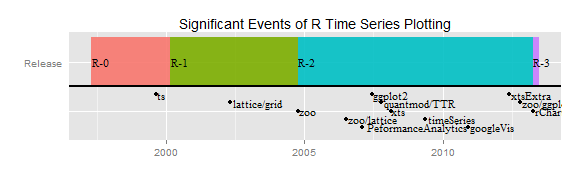
\includegraphics[width=14cm]{timeline}
  \caption{Significant Events of R Time Series Plotting}
  \label{figure:timeline}
\end{figure}

Several packages are worth describing in more detail as these create
much of the foundation of R in Finance currently:

\subsection{quantmod / TTR}\label{quantmod-ttr}

The \emph{``Quantitative Financial Modelling \& Trading Framework for
R''} or \texttt{quantmod} package and the \emph{``Technical Trading
Rules''} or \texttt{TTR} package includes mechanisms to retrieve,
compute, and visualize financial data using the most popular technical
trading rules.

\subsection{xts / zoo}\label{xts-zoo}

The \emph{``Extensible Time Series''} or \texttt{xts} package along with
the \texttt{zoo} package includes mechanisms for the handling of time
series data. Most importantly, the \texttt{xts} package created a
cross-package mechanism for handling the various time-series data
structures, in the process solving a major shortcoming by managing all
time series objects under one class, \texttt{xts}. Additionally, the
package includes functionality to subset and plot time-based objects
using \texttt{zoo}.

\subsection{PerformanceAnalytics}\label{performanceanalytics}

The \texttt{PerformanceAnalytics} package includes a large collection of
econometric functions for financial performance analysis, many of which
are described in \emph{``Practical Portfolio Performance Measurement and
Attribution''} by Carl Bacon. These functions enable analysis of
individual asset and portfolio (aggregation of multiple assets) returns
using popular statistical methods for measuring performance.

\section{New Tools: tidyverse}\label{new-tools-tidyverse}

In parallel, with the progress being made within the R in Finance
community, developers at RStudio have been working to provide useful
tools for data science in R, namely the \texttt{tidyverse}. These
include several packages worth describing in more detail.

\subsection{dplyr / tidyr}\label{dplyr-tidyr}

The \texttt{dplyr} and \texttt{tidyr} packages provide tools to clean
and manipulate data using the \emph{``split-apply-combine''} framework
popularized by Hadley Wickham in ``The Split-Apply-Combine Strategy for
Data Analysis''. The major advances were twofold. First, the packages
simplified and made consistent many of the most common data manipulation
tasks in R. Second and arguably more importantly, the packages
incorporated the use of the pipe (\texttt{\%\textgreater{}\%}) from the
\texttt{magrittr} package enabling the functional verbs to follow an
easy, efficient, and human-readable workflow.

\subsection{purrr}\label{purrr}

The \texttt{purrr} package provides tools for applying functions to data
frames. Similar to the traditional, \texttt{lapply} function,
\texttt{purrr} enables mapping functions within a data frame. The major
advance is that analysis can be performed with ``nested'' data frames
allowing users to keep the entire data analysis workflow in one tidy
data frame.

\subsection{tibble}\label{tibble}

The \texttt{tibble} package extends the traditional \texttt{data.frame}
object by providing useful tools for creating and coercing objects to
``tibbles'' or tidy data frames.

\subsection{ggplot2}\label{ggplot2}

The \texttt{ggplot2} package provides a method of creating complex
visualizations using a layered approach called the ``grammar of
graphics'', which is discussed in {[}INSERT REF{]}. The \texttt{ggplot2}
package has become the dominant form of creating static graphics in the
``tidy'' ecosystem.

{[}ref{]}

\subsection{lubridate}\label{lubridate}

The \texttt{lubridate} package includes functions to manage date and
date-time objects in R, which is essential for working with time series.

{[}ref{]}

\section{Divergent Philosophies, Each with
Advantages}\label{divergent-philosophies-each-with-advantages}

All of the major finance packages work with the \texttt{xts} system,
which is specifically designed for time series analysis. The system
works very well. The extensible time series, ``xts'', data structure was
designed solely for time series analysis. The data structure is much
like a numeric matrix, the only major difference being row names
consisting of the date or date-time information. The advantage to
``xts'' objects is the ability to manage numeric data with date or
date-time references. The objects can be subset or transformed to
different periodicity very easily. The disadvantage is the application
is very strict to numeric data, but because of its focus it manages the
time series data extremely well.

Much of the recent innovation in data analysis has occurred within the
tidy ecosystem. With the entrance of the \texttt{tidyverse}, scaling
analysis using the \emph{``split-apply-combine''} framework has become
easy, efficient, and core functionality. Further, advances in date and
date-time functionality has enabled management of time series data
within the ``tibble'' (``tidy'' data frame) data structure. As the data
science field grows, more innovative functionality will continue to be
developed within the ``tidy'' ecosystem, much of which will be (and is
already) useful to the field of financial analysis.

The two systems, \texttt{xts} and the \texttt{tidyverse}, are very
different on a fundamental and philosophical level. Both have advantages
that are needed within the realm of financial analysis, but
unfortunately the two systems do not work well together. The ``xts''
system is strictly numeric-based, while the ``tidy'' system is strictly
data frame-based. Passing data between systems is difficult if not
painful, and without communication between each the full potential of
financial analysis within R is limited.

To solve this problem, the \texttt{tidyquant} package was developed as a
way to consolidate many of the financial analysis packages within the
\texttt{tidyverse}. In the next section, the
\emph{``split-apply-combine''} framework is discussed conceptually using
non-financial data, and then a demonstration of the \texttt{tidyquant}
package is presented to illustrate some of the key benefits to the
integration of financial packages into the ``tidy'' ecosystem within the
realm of financial analysis.

\section{Split-Apply-Combine
Concepts}\label{split-apply-combine-concepts}

The \emph{``split-apply-combine''} framework is discussed at length in
{[}INSERT REF{]}. To summarize, the core concept is to split a data set
into groups, apply functional analysis, and then recombine. The value in
this approach is the framework enables scaling analyses from one group
to many groups and comparing each group to each other. Rather than
discuss in terms of theory, an example using the \texttt{mtcars} data
set is a better illustration of the \emph{``split-apply-combine''}
framework.

Start with a question:

\begin{quote}
How does engine size affect fuel consumption?
\end{quote}

Load the \texttt{tidyverse} and the \texttt{mtcars} data set in R.

\begin{Schunk}
\begin{Sinput}
library(tidyverse)
data("mtcars")
\end{Sinput}
\end{Schunk}

Next, view the data set. The \texttt{as\_tibble} function is used to
convert to the ``tidy'' data frame structure. The data set consists of
32 rows of data related to various automobiles. Some of the data is
categorical, which can be grouped on.

\begin{Schunk}
\begin{Sinput}
mtcars <- as_tibble(mtcars)
mtcars
\end{Sinput}
\begin{Soutput}
#> # A tibble: 32 × 11
#>      mpg   cyl  disp    hp  drat    wt  qsec    vs    am  gear  carb
#> *  <dbl> <dbl> <dbl> <dbl> <dbl> <dbl> <dbl> <dbl> <dbl> <dbl> <dbl>
#> 1   21.0     6 160.0   110  3.90 2.620 16.46     0     1     4     4
#> 2   21.0     6 160.0   110  3.90 2.875 17.02     0     1     4     4
#> 3   22.8     4 108.0    93  3.85 2.320 18.61     1     1     4     1
#> 4   21.4     6 258.0   110  3.08 3.215 19.44     1     0     3     1
#> 5   18.7     8 360.0   175  3.15 3.440 17.02     0     0     3     2
#> 6   18.1     6 225.0   105  2.76 3.460 20.22     1     0     3     1
#> 7   14.3     8 360.0   245  3.21 3.570 15.84     0     0     3     4
#> 8   24.4     4 146.7    62  3.69 3.190 20.00     1     0     4     2
#> 9   22.8     4 140.8    95  3.92 3.150 22.90     1     0     4     2
#> 10  19.2     6 167.6   123  3.92 3.440 18.30     1     0     4     4
#> # ... with 22 more rows
\end{Soutput}
\end{Schunk}

Many solutions exist to compare fuel consumption and engine size. For
simplicity, the mean and standard deviation are used to characterize the
relationship between number of cylinders, ``cyl'', and miles per gallon,
``mpg''. Implementing \emph{``split-apply-combine''} is as easy as
grouping by a categorical variable and summarizing by the target
measure.

\begin{Schunk}
\begin{Sinput}
mtcars %>%
    mutate(cyl = factor(cyl)) %>%
    group_by(cyl) %>%
    summarize(mpg.mean = mean(mpg),
              mpg.sd = sd(mpg))
\end{Sinput}
\begin{Soutput}
#> # A tibble: 3 × 3
#>      cyl mpg.mean   mpg.sd
#>   <fctr>    <dbl>    <dbl>
#> 1      4 26.66364 4.509828
#> 2      6 19.74286 1.453567
#> 3      8 15.10000 2.560048
\end{Soutput}
\end{Schunk}

From the results, the vehicles, when grouped by ``cyl'', appear to have
an inverse relationship between number of cylinders and miles per
gallon. We can also visualize this relationship using \texttt{ggplot2}.

\begin{Schunk}
\begin{Sinput}
mtcars %>%
    mutate(cyl = factor(cyl)) %>%
    ggplot(aes(x = cyl, y = mpg, fill = cyl)) +
    geom_boxplot() +
    labs(title = "Summarizing Relationships using Split-Apply-Combine",
         subtitle = "ggplot2 Creates Powerful Visualizations")
\end{Sinput}


\begin{center}\includegraphics{RinFinanceDRAFT_files/figure-latex/unnamed-chunk-6-1} \end{center}

\end{Schunk}

Using the \emph{``split-apply-combine''} framework is easy to implement,
but how does it improve financial analysis? Onto more applicable
examples to the realm of financial analysis.

\section{Split-Apply-Combine Applications in
Finance}\label{split-apply-combine-applications-in-finance}

As stated previously, the financial analysis packages do not work well
within the ``tidy'' ecosystem. A new tool is needed, \texttt{tidyquant}.
\textbf{The \texttt{tidyquant} package has one major advance: it
integrates the major financial packages with the \texttt{tidyverse} to
enable the ``tidy'' ecosystem functionality to be applied to financial
data.} The innovation is relatively minor on a conceptual level, but the
net effect is significant in that the tools within the ``tidy''
ecosystem are now unlocked for financial analysis.

\subsection{Example 1: Evaluating Risk vs
Reward}\label{example-1-evaluating-risk-vs-reward}

Start with a question:

\begin{quote}
How does the stock market value risk versus reward?
\end{quote}

This is vague, but answerable by comparing stock returns. Risk is
typically associated with volatility, which can be measured in one way
by standard deviation. Reward is measured by overall returns, which can
be measured by averaging returns over many periods. To start, load
\texttt{tidyquant}, which loads all of the packages needed to evaluate
risk versus reward.

\begin{Schunk}
\begin{Sinput}
# Loads tidyquant, tidyverse, lubridate, quantmod, TTR, xts, zoo, PerformanceAnalytics
library(tidyquant)
\end{Sinput}
\end{Schunk}

Next, collect some financial data. The question implies that a large
sample of stock data is needed to evaluate how performance and risk is
valued within the ``market''. The S\&P 500 index is a good place to
start. \texttt{tidyquant} includes a function, \texttt{tq\_index}, which
returns the stock symbols and company names within an index.

\begin{Schunk}
\begin{Sinput}
sp500 <- tq_index("SP500")
sp500
\end{Sinput}
\end{Schunk}

\begin{Schunk}
\begin{Soutput}
#> # A tibble: 502 × 2
#>    symbol                   company
#>     <chr>                     <chr>
#> 1     MMM                        3M
#> 2     ABT       ABBOTT LABORATORIES
#> 3    ABBV                ABBVIE INC
#> 4     ACN                 ACCENTURE
#> 5    ATVI       ACTIVISION BLIZZARD
#> 6     AYI             ACUITY BRANDS
#> 7    ADBE             ADOBE SYSTEMS
#> 8     AAP        ADVANCE AUTO PARTS
#> 9     AET                     AETNA
#> 10    AMG AFFILIATED MANAGERS GROUP
#> # ... with 492 more rows
\end{Soutput}
\end{Schunk}

Next, the stock prices are easy to retrieve with \texttt{tq\_get}, using
the ``get'' option, \texttt{get\ =\ "stock.prices"}. \texttt{tq\_get} is
a wrapper for \texttt{quantmod::getSymbols}, which enables passing the
underlying function parameters \texttt{from} and \texttt{to}. The input
to \texttt{tq\_get} is \texttt{data}, which can be a single stock
symbol, a vector of stock symbols, or a data frame with stock symbols in
the first column. The latter is passed to \texttt{tq\_get} using the
pipe (\texttt{\%\textgreater{}\%}). The function may take a few minutes
to run because it is downloading the past ten years of daily open, high,
low, close, volume, and adjusted stock prices for the entire S\&P 500
index into one ``tidy'' data frame. It appears that the prices were
retrieved in entirety. The ``tibble'' has 1,205,845 rows and 502 unique
symbols.

\begin{Schunk}
\begin{Sinput}
stock_prices <- sp500 %>%
    tq_get(get  = "stock.prices", 
           from = "2007-01-01", 
           to   = "2017-01-01")
sp500_stock_prices
\end{Sinput}
\end{Schunk}

\begin{Schunk}
\begin{Soutput}
#> # A tibble: 1,205,845 × 9
#>    symbol company       date  open  high   low close  volume adjusted
#>     <chr>   <chr>     <date> <dbl> <dbl> <dbl> <dbl>   <dbl>    <dbl>
#> 1     MMM      3M 2007-01-03 77.53 78.85 77.38 78.26 3781500 60.31064
#> 2     MMM      3M 2007-01-04 78.40 78.41 77.45 77.95 2968400 60.07174
#> 3     MMM      3M 2007-01-05 77.89 77.90 77.01 77.42 2765200 59.66330
#> 4     MMM      3M 2007-01-08 77.42 78.04 76.97 77.59 2434500 59.79431
#> 5     MMM      3M 2007-01-09 78.00 78.23 77.44 77.68 1896800 59.86367
#> 6     MMM      3M 2007-01-10 77.31 77.96 77.04 77.85 1787500 59.99468
#> 7     MMM      3M 2007-01-11 78.05 79.03 77.88 78.65 2372500 60.61120
#> 8     MMM      3M 2007-01-12 78.41 79.50 78.22 79.36 2582200 61.15835
#> 9     MMM      3M 2007-01-16 79.48 79.62 78.92 79.56 2526600 61.31248
#> 10    MMM      3M 2007-01-17 79.33 79.51 78.75 78.91 2711300 60.81156
#> # ... with 1,205,835 more rows
\end{Soutput}
\end{Schunk}

Next, the \emph{``split-apply-combine''} framework is used to group the
prices by stock symbol and to calculate the logarithmic daily returns.
The log returns are used to create a more ``normal'' distribution. The
transform is applied using \texttt{tq\_transform}, which is used in
situations where periodicity changes (or can change). The
\texttt{quantmod} OHLC (open, high, low, close) notation is used to
collect the adjusted prices (\texttt{ohlc\_fun\ =\ Ad}) and send these
prices to the \texttt{periodReturn} function
(\texttt{transform\_fun\ =\ periodReturn}). The additional arguments,
\texttt{period\ =\ "daily"} and \texttt{type\ =\ "log"} are passed to
the transformation function, which is \texttt{periodReturn}. The
\texttt{col\_rename\ =\ "dlr"} is a quick renaming function for the
output column. In this case, ``dlr'' refers to daily log returns. The
daily log returns for each of the 502 stock symbols is generated below.

\begin{Schunk}
\begin{Sinput}
sp500_returns <- sp500_stock_prices %>%
    group_by(symbol) %>%
    tq_transform(ohlc_fun = Ad, transform_fun = periodReturn, 
                 period = "daily", type = "log", col_rename = "dlr")
sp500_returns
\end{Sinput}
\end{Schunk}

\begin{Schunk}
\begin{Soutput}
#> Source: local data frame [1,205,845 x 3]
#> Groups: symbol [502]
#> 
#>    symbol       date          dlr
#>     <chr>     <date>        <dbl>
#> 1     MMM 2007-01-03  0.000000000
#> 2     MMM 2007-01-04 -0.003969091
#> 3     MMM 2007-01-05 -0.006822440
#> 4     MMM 2007-01-08  0.002193382
#> 5     MMM 2007-01-09  0.001159338
#> 6     MMM 2007-01-10  0.002186048
#> 7     MMM 2007-01-11  0.010223770
#> 8     MMM 2007-01-12  0.008986823
#> 9     MMM 2007-01-16  0.002516944
#> 10    MMM 2007-01-17 -0.008203410
#> # ... with 1,205,835 more rows
\end{Soutput}
\end{Schunk}

Next, the mean and standard deviation of the daily log returns are used
to evaluate and compare the stocks. The easiest way is to use
\texttt{tq\_performance}, which enables applying the
\texttt{PerformanceAnalytics} performance functions to ``tidy'' data
frames of asset or portfolio returns. The \texttt{table.Stats} function
returns the arithmetic mean and standard deviation along with a number
of other useful statistics that characterize the returns.

\begin{Schunk}
\begin{Sinput}
sp500_stats <- sp500_returns %>%
    tq_performance(Ra = dlr, performance_fun = table.Stats, ci = 0.95, digits = 6) 
sp500_stats
\end{Sinput}
\end{Schunk}

\begin{Schunk}
\begin{Soutput}
#> Source: local data frame [502 x 17]
#> Groups: symbol [502]
#> 
#>    symbol ArithmeticMean GeometricMean  Kurtosis `LCLMean(0.95)`  Maximum
#>     <chr>          <dbl>         <dbl>     <dbl>           <dbl>    <dbl>
#> 1     MMM       0.000431      0.000331  5.806040       -0.000120 0.094204
#> 2     ABT       0.000302      0.000215  6.294066       -0.000211 0.091903
#> 3    ABBV       0.000714      0.000565  3.868658       -0.000350 0.095982
#> 4     ACN       0.000543      0.000404  8.532566       -0.000108 0.151577
#> 5    ATVI       0.000604      0.000359 10.735599       -0.000263 0.209206
#> 6     AYI       0.000701      0.000420  6.011008       -0.000225 0.161304
#> 7    ADBE       0.000376      0.000147  8.992646       -0.000457 0.134165
#> 8     AAP       0.000634      0.000430 14.825940       -0.000156 0.153215
#> 9     AET       0.000453      0.000208  7.370411       -0.000410 0.163419
#> 10    AMG       0.000126     -0.000289  8.848371       -0.000996 0.211618
#> # ... with 492 more rows, and 11 more variables: Median <dbl>,
#> #   Minimum <dbl>, NAs <dbl>, Observations <dbl>, Quartile1 <dbl>,
#> #   Quartile3 <dbl>, SEMean <dbl>, Skewness <dbl>, Stdev <dbl>,
#> #   `UCLMean(0.95)` <dbl>, Variance <dbl>
\end{Soutput}
\end{Schunk}

Finally, we have the tools to visualize risk versus reward. Risk can be
characterized by the standard deviation, or volatility, and reward can
be characterized by average returns. A plot of MDLR versus SDDLR shows
the relationship. The market tends to penalize stocks with higher
standard deviations of daily log returns (SDDLR), or in other words more
volatility.

\begin{Schunk}
\begin{Sinput}
sp500_stats %>%
    filter(Observations >= 252 * 5) %>%
    ggplot(aes(x = Stdev, y = ArithmeticMean, col = (ArithmeticMean / Stdev))) +
    geom_point() +
    geom_smooth(method = "lm") +
    labs(title = "Evaluating Risk Vs Reward for Stocks in the SP500 Index",
         subtitle = "Split-Apply-Combine Enables Scaling Financial Analysis",
         caption = "Looks like an inverse relationship exists between MDLR and SDDLR",
         x = "Standard Deviation of Daily Log Returns (SDDLR)",
         y = "Arithmetic Mean of Daily Log Returns (MDLR)") +
    theme_tq()
\end{Sinput}


\begin{center}\includegraphics{RinFinanceDRAFT_files/figure-latex/unnamed-chunk-16-1} \end{center}

\end{Schunk}

\subsection{Example 2: Visualizing Portfolio
Performance}\label{example-2-visualizing-portfolio-performance}

Portfolio aggregation is a useful technique to reduce risk while
maintaining returns. In this example, the goal is to evaluate a few
blended portfolios of ``FANG'' stocks (``FB'', ``AMZN'', ``NFLX'',
``GOOG'' popularized by Jim Cramer). The following portfolio blends will
be evaluated:

\begin{itemize}
\tightlist
\item
  Portfolio 1: 50\% FB, 25\% AMZN, 25\% NFLX, 0\% GOOG
\item
  Portfolio 2: 0\% FB, 50\% AMZN, 25\% NFLX, 25\% GOOG
\item
  Portfolio 3: 25\% FB, 0\% AMZN, 50\% NFLX, 25\% GOOG
\item
  Portfolio 4: 25\% FB, 25\% AMZN, 0\% NFLX, 50\% GOOG
\end{itemize}

First, collect the data for the ``FANG'' stocks.

\begin{Schunk}
\begin{Sinput}
FANG <- c("FB", "AMZN", "GOOG", "NFLX") %>%
    tq_get(get = "stock.prices",
           from = "2007-01-01",
           to   = "2017-01-01")
FANG
\end{Sinput}
\end{Schunk}

\begin{Schunk}
\begin{Soutput}
#> # A tibble: 8,717 × 8
#>    symbol       date  open  high   low close    volume adjusted
#>     <chr>     <date> <dbl> <dbl> <dbl> <dbl>     <dbl>    <dbl>
#> 1      FB 2012-05-18 42.05 45.00 38.00 38.23 573576400    38.23
#> 2      FB 2012-05-21 36.53 36.66 33.00 34.03 168192700    34.03
#> 3      FB 2012-05-22 32.61 33.59 30.94 31.00 101786600    31.00
#> 4      FB 2012-05-23 31.37 32.50 31.36 32.00  73600000    32.00
#> 5      FB 2012-05-24 32.95 33.21 31.77 33.03  50237200    33.03
#> 6      FB 2012-05-25 32.90 32.95 31.11 31.91  37149800    31.91
#> 7      FB 2012-05-29 31.48 31.69 28.65 28.84  78063400    28.84
#> 8      FB 2012-05-30 28.70 29.55 27.86 28.19  57267900    28.19
#> 9      FB 2012-05-31 28.55 29.67 26.83 29.60 111639200    29.60
#> 10     FB 2012-06-01 28.89 29.15 27.39 27.72  41855500    27.72
#> # ... with 8,707 more rows
\end{Soutput}
\end{Schunk}

Next, transform to monthly returns using the
\emph{``split-apply-combine''} framework. Use \texttt{group\_by} to
group on the ``symbol'' column, and \texttt{tq\_transform} to transform
the adjusted prices to monthly arithmetic returns. Note that ``FB'' was
actively traded for a full year beginning in 2013, so it makes sense to
compare the investments since then.

\begin{Schunk}
\begin{Sinput}
FANG_returns <- FANG %>%
    filter(date >= ymd("2013-01-01")) %>%
    group_by(symbol) %>%
    tq_transform(ohlc_fun = Ad,
                 transform_fun = periodReturn,
                 period = "monthly",
                 col_rename = "returns")
FANG_returns
\end{Sinput}
\begin{Soutput}
#> Source: local data frame [192 x 3]
#> Groups: symbol [4]
#> 
#>    symbol       date       returns
#>     <chr>     <date>         <dbl>
#> 1      FB 2013-01-31  0.1064285714
#> 2      FB 2013-02-28 -0.1204002582
#> 3      FB 2013-03-28 -0.0612844037
#> 4      FB 2013-04-30  0.0856137608
#> 5      FB 2013-05-31 -0.1231544833
#> 6      FB 2013-06-28  0.0217658727
#> 7      FB 2013-07-31  0.4790996977
#> 8      FB 2013-08-30  0.1220109272
#> 9      FB 2013-09-30  0.2165172871
#> 10     FB 2013-10-31 -0.0003981883
#> # ... with 182 more rows
\end{Soutput}
\end{Schunk}

\subsubsection{Individual Asset
Performance}\label{individual-asset-performance}

Before the portfolios are generated, it makes sense to visualize and
assess the performance of the individual asset returns. NFLX is the best
performer, but it also makes sense to investigate risk.

\begin{Schunk}
\begin{Sinput}
init_investment <- 10000
FANG_wealth <- FANG_returns %>%
    mutate(wealth.index = init_investment * cumprod(1 + returns))

FANG_wealth %>%
    ggplot(aes(x = date, y = wealth.index, color = symbol)) +
    geom_line(size = 2) +
    geom_smooth(method = "loess") +
    labs(title = "Individual Stocks: Comparing the Growth of 10K", x = "", y = "Investment Value")
\end{Sinput}


\begin{center}\includegraphics{RinFinanceDRAFT_files/figure-latex/unnamed-chunk-20-1} \end{center}

\end{Schunk}

Use \texttt{tq\_performance} with another table function,
\texttt{table.DownsideRisk}, to estimate risk measures across the FANG
stocks. While NFLX returns are stellar the risk is also very high.

\begin{Schunk}
\begin{Sinput}
FANG_returns %>%
    tq_performance(Ra = returns, Rb = NULL, performance_fun = table.DownsideRisk)
\end{Sinput}
\begin{Soutput}
#> Source: local data frame [4 x 12]
#> Groups: symbol [4]
#> 
#>   symbol `DownsideDeviation(0%)` `DownsideDeviation(MAR=10%)`
#>    <chr>                   <dbl>                        <dbl>
#> 1     FB                  0.0390                       0.0430
#> 2   AMZN                  0.0391                       0.0436
#> 3   GOOG                  0.0251                       0.0296
#> 4   NFLX                  0.0631                       0.0673
#> # ... with 9 more variables: `DownsideDeviation(Rf=0%)` <dbl>,
#> #   GainDeviation <dbl>, `HistoricalES(95%)` <dbl>,
#> #   `HistoricalVaR(95%)` <dbl>, LossDeviation <dbl>,
#> #   MaximumDrawdown <dbl>, `ModifiedES(95%)` <dbl>,
#> #   `ModifiedVaR(95%)` <dbl>, SemiDeviation <dbl>
\end{Soutput}
\end{Schunk}

\subsubsection{Portfolio Performance}\label{portfolio-performance}

Now onto portfolios. The stocks returns need to be aggregated, which
takes three steps:

\begin{enumerate}
\def\labelenumi{\arabic{enumi}.}
\tightlist
\item
  Make a portfolio by repeating the stock returns
\item
  Create a weights table to map weights of various portfolios
\item
  Aggregate the portfolios using \texttt{tq\_portfolio}, a wrapper for
  \texttt{PerformanceAnalytics::Return.portfolio}
\end{enumerate}

\paragraph{Step 1: Make a portfolio by repeating the stock
returns}\label{step-1-make-a-portfolio-by-repeating-the-stock-returns}

Use \texttt{tq\_repeat\_df} to repeat \texttt{n\ =\ 4} times. This
function grows the data frame length-wise, adding an index column named
``portfolio'', and grouping by ``portfolio''. We now have four groups
that will be used as portfolios.

\begin{Schunk}
\begin{Sinput}
FANG_returns_mult <- FANG_returns %>%
    tq_repeat_df(n = 4)
FANG_returns_mult
\end{Sinput}
\begin{Soutput}
#> Source: local data frame [768 x 4]
#> Groups: portfolio [4]
#> 
#>    portfolio symbol       date       returns
#>        <int>  <chr>     <date>         <dbl>
#> 1          1     FB 2013-01-31  0.1064285714
#> 2          1     FB 2013-02-28 -0.1204002582
#> 3          1     FB 2013-03-28 -0.0612844037
#> 4          1     FB 2013-04-30  0.0856137608
#> 5          1     FB 2013-05-31 -0.1231544833
#> 6          1     FB 2013-06-28  0.0217658727
#> 7          1     FB 2013-07-31  0.4790996977
#> 8          1     FB 2013-08-30  0.1220109272
#> 9          1     FB 2013-09-30  0.2165172871
#> 10         1     FB 2013-10-31 -0.0003981883
#> # ... with 758 more rows
\end{Soutput}
\end{Schunk}

\paragraph{Step 2: Create a Weights Table to Map
Weights}\label{step-2-create-a-weights-table-to-map-weights}

Constructing a weights table using the portfolio blending parameters:

\begin{itemize}
\tightlist
\item
  Portfolio 1: 50\% FB, 25\% AMZN, 25\% NFLX, 0\% GOOG
\item
  Portfolio 2: 0\% FB, 50\% AMZN, 25\% NFLX, 25\% GOOG
\item
  Portfolio 3: 25\% FB, 0\% AMZN, 50\% NFLX, 25\% GOOG
\item
  Portfolio 4: 25\% FB, 25\% AMZN, 0\% NFLX, 50\% GOOG
\end{itemize}

\begin{Schunk}
\begin{Sinput}
weights_table <- tribble(
    ~portfolio, ~stocks, ~weights,
    1,          "FB",    0.50,
    1,          "AMZN",  0.25,
    1,          "NFLX",  0.25,
    1,          "GOOG",  0.00,

    2,          "FB",    0.00,
    2,          "AMZN",  0.50,
    2,          "NFLX",  0.25,
    2,          "GOOG",  0.25,

    3,          "FB",    0.25,
    3,          "AMZN",  0.00,
    3,          "NFLX",  0.50,
    3,          "GOOG",  0.25,

    4,          "FB",    0.25,
    4,          "AMZN",  0.25,
    4,          "NFLX",  0.00,
    4,          "GOOG",  0.50) %>%
    group_by(portfolio)
weights_table
\end{Sinput}
\begin{Soutput}
#> Source: local data frame [16 x 3]
#> Groups: portfolio [4]
#> 
#>    portfolio stocks weights
#>        <dbl>  <chr>   <dbl>
#> 1          1     FB    0.50
#> 2          1   AMZN    0.25
#> 3          1   NFLX    0.25
#> 4          1   GOOG    0.00
#> 5          2     FB    0.00
#> 6          2   AMZN    0.50
#> 7          2   NFLX    0.25
#> 8          2   GOOG    0.25
#> 9          3     FB    0.25
#> 10         3   AMZN    0.00
#> 11         3   NFLX    0.50
#> 12         3   GOOG    0.25
#> 13         4     FB    0.25
#> 14         4   AMZN    0.25
#> 15         4   NFLX    0.00
#> 16         4   GOOG    0.50
\end{Soutput}
\end{Schunk}

\paragraph{Step 3: Aggregate the Portfolios with
tq\_portfolio}\label{step-3-aggregate-the-portfolios-with-tq_portfolio}

Aggregating portfolio using \texttt{tq\_portfolio}, a wrapper for
\texttt{PerformanceAnalytics::Return.portfolio}. The
\texttt{Return.portfolio} has additional arguments to create a wealth
index, which is the compounded return. Setting
\texttt{wealth.index\ =\ TRUE} and multiplying the result by the initial
investment value of \$10,000 returns a wealth index.

\begin{Schunk}
\begin{Sinput}
# C: Aggregate portfolio with tq_portfolio. Pass wealth.index = TRUE
init_investment <- 10000
FANG_portfolio_wealth <- FANG_returns_mult %>%
    tq_portfolio(assets_col = symbol, returns_col = returns,
                 weights = weights_table, wealth.index = TRUE,
                 col_rename = "wealth.index") %>%
    mutate(wealth.index = wealth.index * init_investment)
\end{Sinput}
\end{Schunk}

Next, we can visualize the performance of the various blended
portfolios.

\begin{Schunk}
\begin{Sinput}
FANG_portfolio_wealth  %>%
    ggplot(aes(x = date, y = wealth.index, color = factor(portfolio))) +
    geom_line(size = 2) +
    geom_smooth(method = "loess") +
    labs(title = "Portfolios: Comparing the Growth of 10K",
         subtitle = "Quickly visualize blended portfolio performance",
         x = "", y = "Investment Value",
         color = "Portfolio Number: ") +
    theme_tq() +
    scale_color_tq() +
    scale_y_continuous(labels = scales::dollar)
\end{Sinput}


\begin{center}\includegraphics{RinFinanceDRAFT_files/figure-latex/unnamed-chunk-25-1} \end{center}

\end{Schunk}

Finally, the risk is assessed in the same manner as the individual
assets. The portfolio aggregation is performed without the
\texttt{wealth.index} option, which aggregates uncompounded returns. The
returns are ``piped'' to the \texttt{tq\_performance} function, which
returns the downside risk table. Portfolio 1 appears to have a good
combination of high returns and low downside risk.

\begin{Schunk}
\begin{Sinput}
FANG_returns_mult %>%
    tq_portfolio(assets_col = symbol, returns_col = returns,
                 weights = weights_table, col_rename = "returns") %>%
    tq_performance(Ra = returns, Rb = NULL, performance_fun = table.DownsideRisk)
\end{Sinput}
\begin{Soutput}
#> Source: local data frame [4 x 12]
#> Groups: portfolio [4]
#> 
#>   portfolio `DownsideDeviation(0%)` `DownsideDeviation(MAR=10%)`
#>       <dbl>                   <dbl>                        <dbl>
#> 1         1                  0.0344                       0.0385
#> 2         2                  0.0423                       0.0465
#> 3         3                  0.0479                       0.0521
#> 4         4                  0.0221                       0.0259
#> # ... with 9 more variables: `DownsideDeviation(Rf=0%)` <dbl>,
#> #   GainDeviation <dbl>, `HistoricalES(95%)` <dbl>,
#> #   `HistoricalVaR(95%)` <dbl>, LossDeviation <dbl>,
#> #   MaximumDrawdown <dbl>, `ModifiedES(95%)` <dbl>,
#> #   `ModifiedVaR(95%)` <dbl>, SemiDeviation <dbl>
\end{Soutput}
\end{Schunk}

\section{Conclusion}\label{conclusion}

\address{%
Matt Dancho\\
Business Science\\
\\
}
\href{mailto:mdancho@business-science.io}{\nolinkurl{mdancho@business-science.io}}

\address{%
Davis Vaughan\\
Business Science\\
\\
}
\href{mailto:dvaughan@business-science.io}{\nolinkurl{dvaughan@business-science.io}}

